\documentclass[a4paper]{article}

% Packages
\usepackage{graphicx}
\usepackage[margin=1in]{geometry}
\usepackage[backend=bibtex]{biblatex}
\usepackage{comment}
\usepackage{hyperref}


\addbibresource{references.bib}

\title{Evaluation of Machine Translation in Languages}
\author{Stefan Liemawan Adji}
\date{\today}

\begin{document}

\maketitle

\section{Introduction}


According to Ethnologue \cite{ethnologue-2024}, 7,164 languages currently exist and in use today, with 40\% of them considered endangered.

As of July 2024, 243 languages and languages varities are supported by Google Translate (according to Wikipedia \cite{wikipedia-google-translate})

Machine translation (MT) has emerged as a pivotal technology in facilitating cross-cultural communication and global information exchange. With the exponential growth of digital content in diverse languages, the demand for accurate and efficient translation systems has never been greater. This paper aims to evaluate and compare the performance of various machine translation models across multiple languages, shedding light on their effectiveness and limitations in real-world applications.

Effective machine translation hinges on the ability of algorithms to comprehend and accurately render meaning from source text in one language to target text in another. Traditionally, statistical methods dominated the landscape, employing linguistic rules and alignment techniques. However, the advent of neural machine translation (NMT) has revolutionized the field, leveraging deep learning architectures to achieve remarkable improvements in translation quality.

Statistical machine translation, which previously dominated MT research for many years with its reliance on various count-based models, has largely been surpassed by neural machine translation (NMT) \cite{stahlberg-2020-nmt-review}.

The languages chosen for evaluation in this study represent a wide overview, striking a balance between resources and diversity.

The evaluation criteria encompass standard metrics such as BLEU (Bilingual Evaluation Understudy) \cite{papieni-2002-bleu}, METEOR (Metric for Evaluation of Translation with Explicit ORdering) \cite{lavie-2007-meteor} to capture nuances in translation quality. These metrics not only quantify the fidelity of translations but also offer insights into the models' adaptability and robustness across different linguistic pairs.

Through simple experimentation and analysis, this paper aims to evaluate existing techniques across different languages
and contribute valuable insights into the current state of machine translation technology. By comparing metrics among languages, I hope to inform future researchers of the effectiveness of machine translation on each individual languages that are included in this paper.


Evaluating languages enhances understanding of linguistic structures, phonetics, syntax, semantics, and other linguistic components. This knowledge contributes to the broader field of linguistics and helps in developing theories about language evolution, language families, and the cognitive processes involved in language acquisition and use.

Machine translation can be tracked to as early as 1949 \cite{weaver-1999}

\section{Related Work}

As is the case of most fields within Natural Language Processing (NLP), the current state-of-the-art (SOTA) in machine translation (MT) is characterised by the significant advancements brought by large language models (LLMs) like OpenAI's GPT-4. These models have surpassed traditional neural machine translation (NMT) systems in several areas, offering more nuanced and accurate translations, especially in handling context and idiomatic expressions.

mBART \cite{liu-2020-mbart} is considered one of the State-of-the-Art as of this moment for multilingual translation.

T5 \cite{raffel-2023-t5}

\section{Tatoeba Dataset}

\subsection{Overview}

Tatoeba is a vast, continuously expanding database consisting sentences and their translations, built through the contributions of thousands of volunteers, offering a tool that allows users to see examples of how words are used in sentences \cite{tatoeba}. They currently have 12,132,349 sentences and 423 supported languages, with around one to two thousand new sentences added daily, on average

\begin{figure}[htbp]
    \centering
    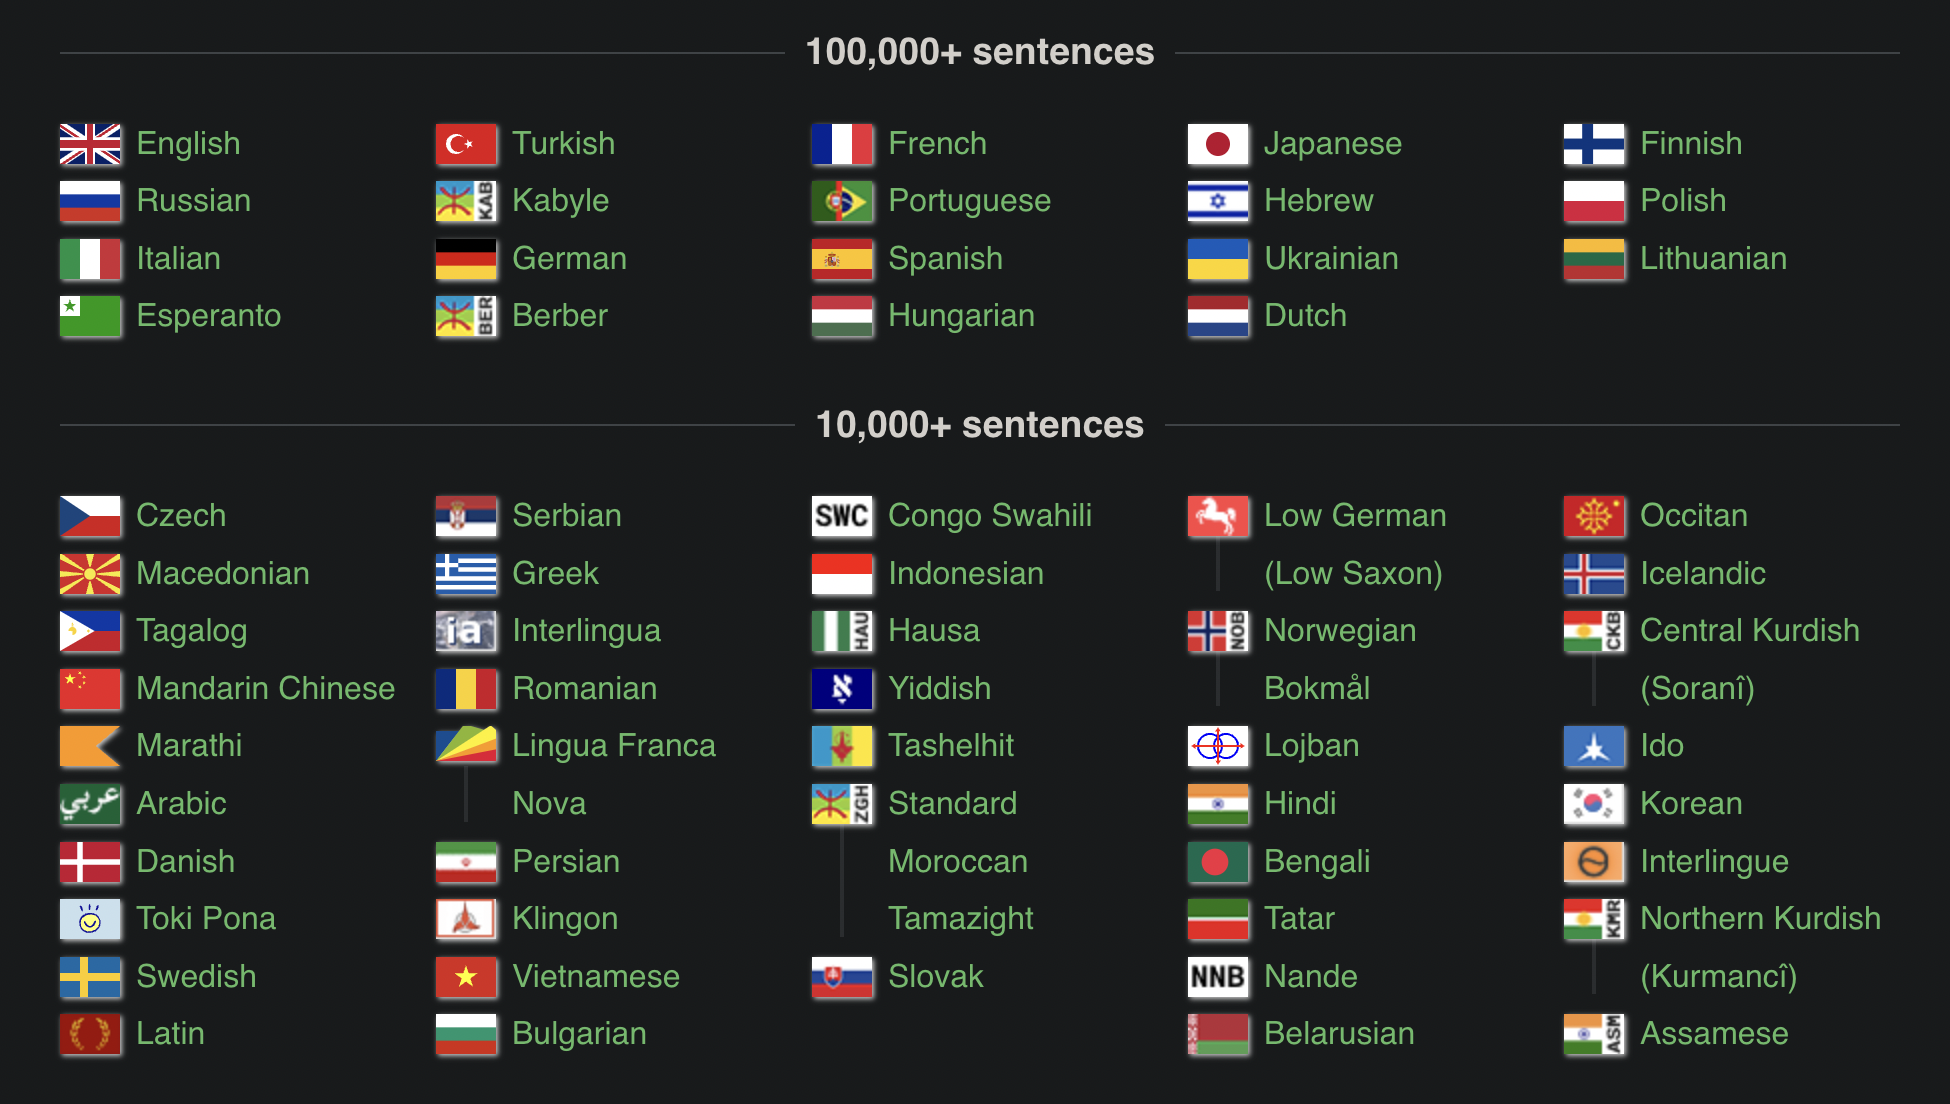
\includegraphics[width=0.9\linewidth]{images/tatoeba_languages.png}
    \caption{Tatoeba languages repository with 10,000+ sentences and 100,000+ sentences \cite{tatoeba}}
    \label{fig:tatoeba_languages}
\end{figure}

Tatoeba English sentence dataset contains 1,905,089 sentences, the largest one in their repository, with Russian in the second place with 1,066,633 sentences. Some of the languages supported in the website is shown in Figure \ref{fig:tatoeba_languages} and Figure \ref{fig:tatoeba_top_bottom_languages}, sorted from the biggest corpus. Low-resource languages such as Rendille, Southern Haida, and Cuyonon can be seen at the bottom of the list, having only a single sentence example. Ancestor languages such as Old Saxon and Old Turkish can also be seen in the list, subsequently with low number of examples.

\begin{figure}[htbp]
    \centering
    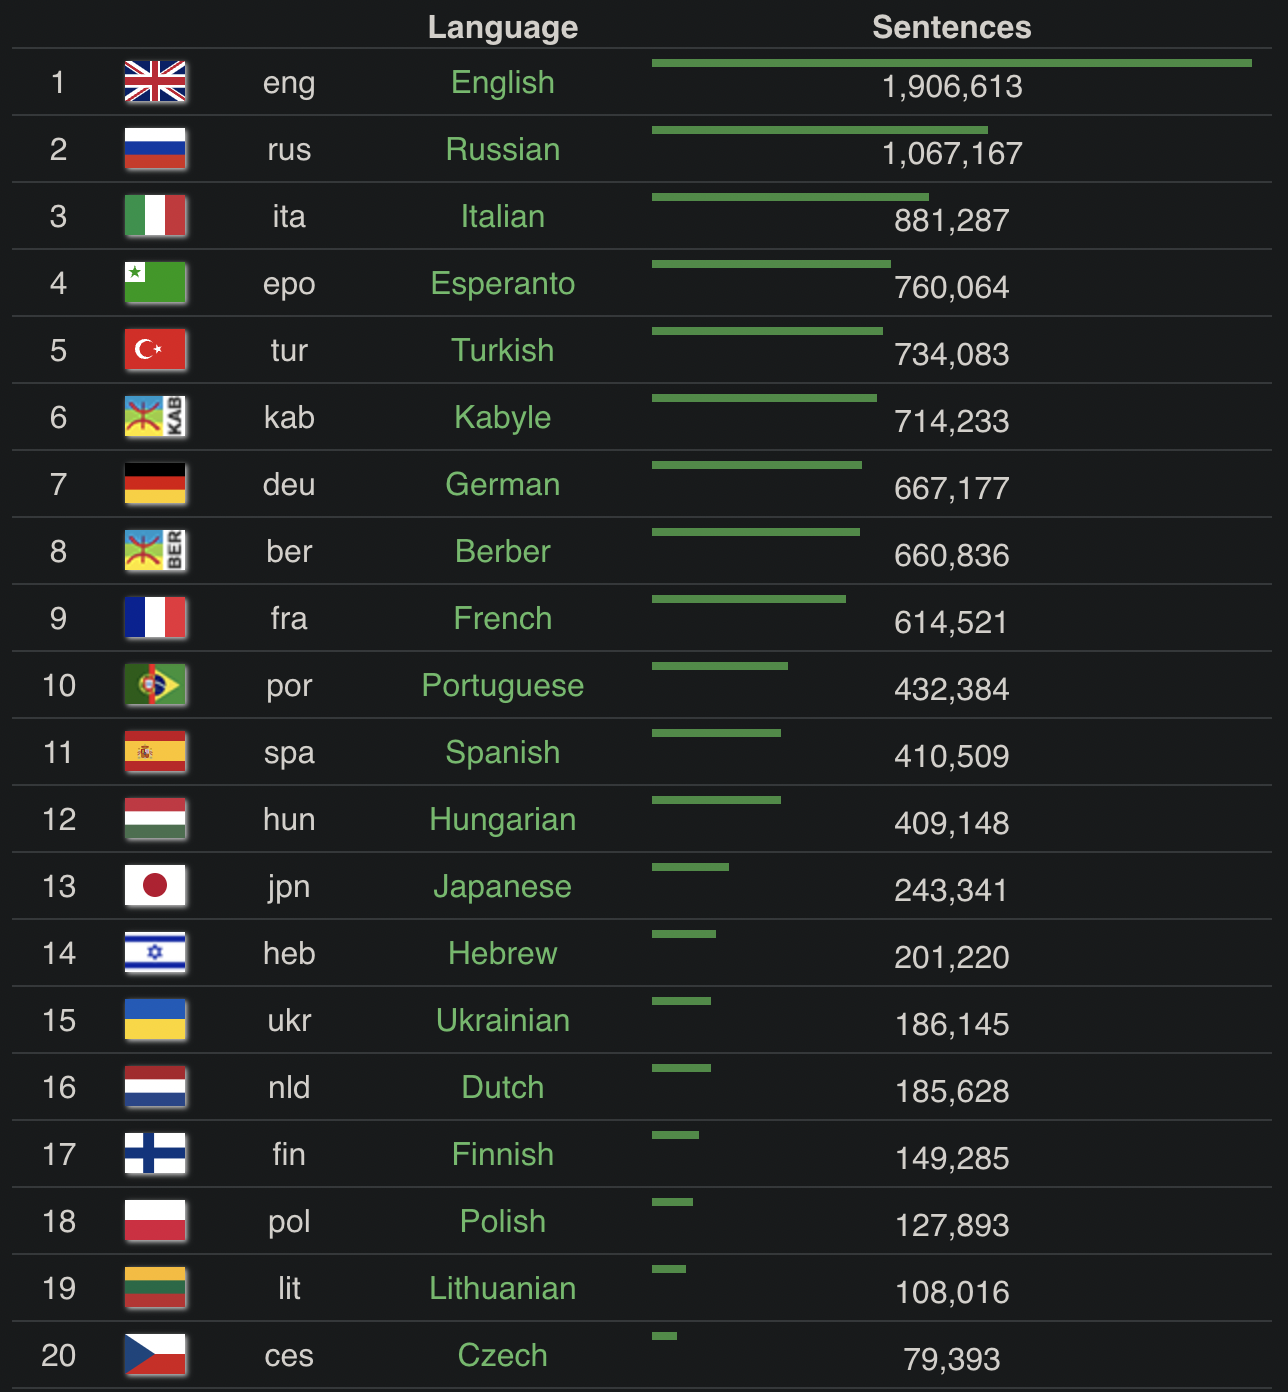
\includegraphics[width=0.5\linewidth]{images/tatoeba_top_20_lang.png}
    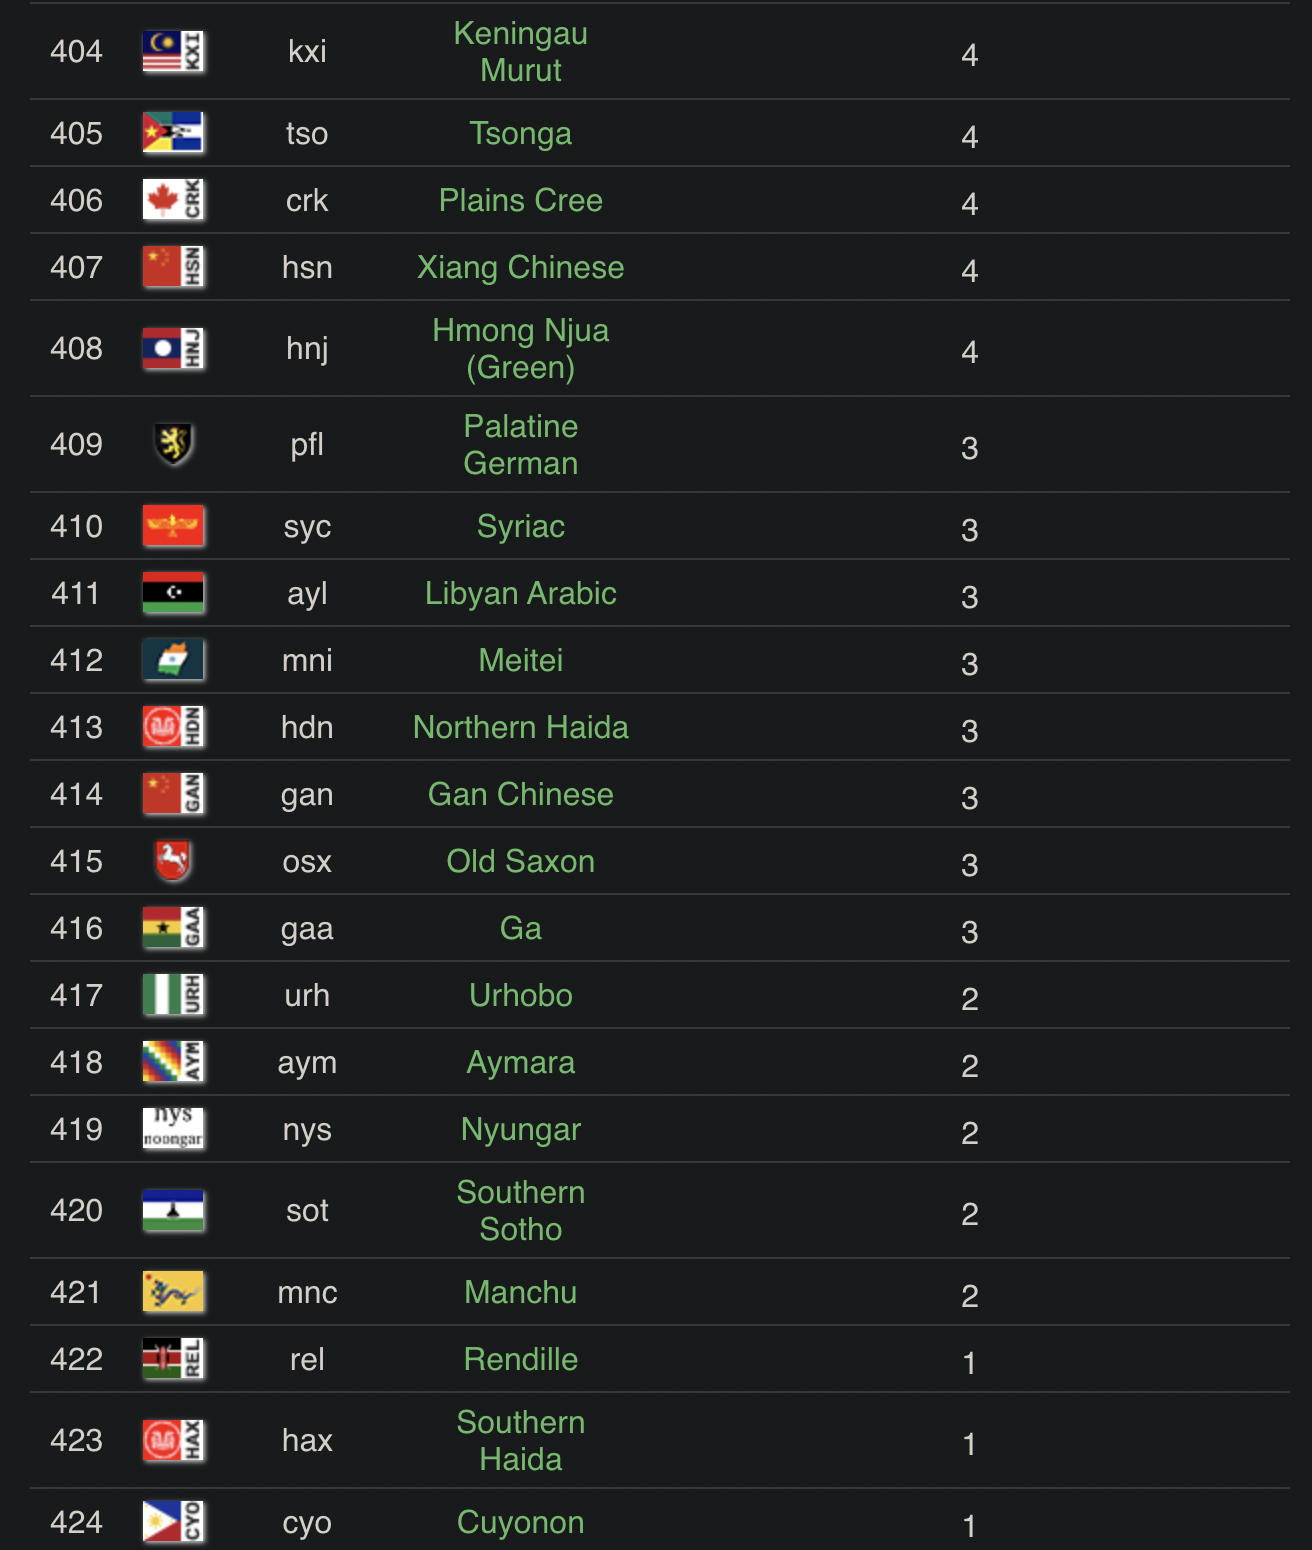
\includegraphics[width=0.46\linewidth]{images/tatoeba_bottom_20_lang.png}
    \caption{Tatoeba top 20 and bottom 20 languages based on sentences count \cite{tatoeba}}
    \label{fig:tatoeba_top_bottom_languages}
\end{figure}


\subsection{Analysis}

Sentences typically consist of everyday phrases such as 'I have to go to sleep', 'That is intriguing', and 'Where do you live?' They may also include single-word exclamations like 'Speak!' or 'Look!' Additionally, multiple sentences such as 'You may write in any language you want. On Tatoeba, all languages are considered equal', and 'Guns don't kill people. People kill people' can be found inside the corpus. A few of them also include human names, 'Compare your answer with Tom's', 'Muiriel is 20 now'. All of the sentences are straightforward and literal, without the use of linguistic devices such as metaphors or sarcasm. Therefore, machine translation process should be straightforward on this level.

\section{Methodology}

Take the list of most spoken language by population according to Wikipedia \cite{wikipedia-list-languages}, then take one for each branch.

Sentences in English are downloaded, 1,898,494 sentences (it is unclear why it is less than the number stated in the Tatoeba website). Then for each langauges, download sentence pairs compared to English. Merge every language sentences into one big dataframe, only keep where sentences exist for every language.

Target language will be English, with machine translation task defined as Many-to-English.

\begin{table}[htbp]
    \centering
    \begin{tabular}{|l|l|}
        \hline
        \textbf{No.} & \textbf{Language} \\
        \hline
        1            & Dutch             \\
        2            & Finnish           \\
        3            & French            \\
        4            & German            \\
        5            & Hebrew            \\
        6            & Hungarian         \\
        7            & Italian           \\
        8            & Japanese          \\
        9            & Mandarin Chinese  \\
        10           & Polish            \\
        11           & Portuguese        \\
        12           & Russian           \\
        13           & Spanish           \\
        14           & Turkish           \\
        15           & Ukrainian         \\
        \hline
    \end{tabular}
    \caption{List of chosen languages for evaluation}
\end{table}

Sentences dataset from Tatoeba is used \footnote{\url{https://tatoeba.org/}}. Languages that has more than fifty thousand sentences are selected. Accordingly, languages that are available for mbart is also selected based on the list here \footnote{\url{https://dl-translate.readthedocs.io/en/latest/available_languages/}}

For translation, all languages are translated into English as the target language. Then compare the true English sentence and the predicted one, calculated BLEU.

\section{Evaluation}

\section{Conclusion}

\printbibliography
\end{document}
